\documentclass{"article"}

\input{../preamble.tex}
\addbibresource{References.bib}

\begin{document}


\section{Einleitung}
In diesem Part der Arbeit, haben wir versucht Musikstücke ihren Komponisten zuzuordnen. Dafür haben wir das Datenset "Classical Music MIDI as CSV", welches auf Kaggle zur Verfügung steht, verwendet.
Auch hier liegt bei den einzelnen Musikstücken wieder nicht die Audiodatei selbst vor, sondern ein MIDI File, mit welchem die Maschine umgehen kann.

Das Datenset ist wiefolgt aufgebaut: 
    Es gibt 10 verschiedene Kategorien, in welche die Musikstücke eingeordnet werden.
    \begin{enumerate}
        \item ALL
        \item Bach
        \item Beethoven
        \item Chopin
        \item Haendel
        \item Mozart
        \item Scarlatti
        \item Schubert
        \item Varios - Título desconocido (spanisch für: "Titel unbekannt")
        \item Vivaldi
    \end{enumerate}

Gibt es zu einem Künstler mehr als 100 Stücke, so hat dieser seine eigene Kategorie (wie z.B. Bach, Mozart, ...). Von vielen Künstlern stehen aber weniger als 100 Werke zur Verfügung.
Diese finden sich alle in der Kategorie "ALL". Solche Künstler sind beispielsweise: Pachelbel, Jakobowski oder Strauss. Weitere Informationen zum Aufbau des Datensets, siehe \parencite{Dataset}.

Über die Stücke selbst liegen wieder verschiedene Informationen, wie beispielsweise die Noten oder der Taxt vor. Für die Klassifikation haben wir nur die Noten verwendet.
Die Noten sind Zahlenwerte von eins bis 127, sprich es ist gleich aufgebaut, wie bei der Generierung.

\section{Theorie}
Noch überlegen.

\section{Klassifikation mit RandomForestClassifier}
\textit{Im Allgemeinen haben wir in diesem Abschnitt die Kategorien 1 (ALL) und 8 (Título desconocido) ausgelassen, weil sie alle Stücke bzw. Stücke ohne Künstler beinhalten und wir das 
für die Klassifikation nicht verwenden können.}
\subsection{Vorbereitung der Daten}

\subsection{Erster Versuch}
Zur Klassifikation verwenden wir einen Random Forest. Nachem wir die Daten vorbereitet haben, ordnen wir die Stücke ihren Komponisten zu.
Da die Daten sehr unausgeglichen sind (so hat zum Beispiel Bach am meisten mit 35.191 Daten und Haendel mit nur 6.031 die wenigsten Informationen) muss das Datenset balanciert werden. 
Dabei gehen aber im schlimmsten Fall (von Bach) 29.160 Datenpunkte, also über 80\% der Informationen verloren. Das ist natürlich nicht gut für die Klassifikation, wie sich später auch zeigen wird.



Trainiert man einen Random Forest mit den Default-Werten (siehe: \parencite{Dataset}), so erhält man eine Accuracy von: 27\%. Also schlecht. Setzt man den Defaultwert von \emph{n\_estimators}, also 
der Anzahl der Bäume im Forest höher, so verbessert sich die Accuracy. Bei beispielsweise 1.000 Bäumen hat man eine Genauigkeit von 31\%, was besser aber immernoch schlecht ist.
Betrachtet man die Confusionmatrix (\ref{fig:Klassifikation_ohne_Epochen}), kann man folgendes erkennen:

\begin{itemize}
    \item Stücke von Schubert können gut klassifiziert werden.
    \item Auf der anderen Seite, fällt es dem Modell schwer Werke von Scarlatti einzuordnen.
    \item Im Allgemeinen sieht man aber, dass Musikstücke oft in der gleichen Zeitepoche, in welcher die Künstler gelebt haben, vertauscht werden.
\end{itemize}

\begin{figure}[h]
  \centering
  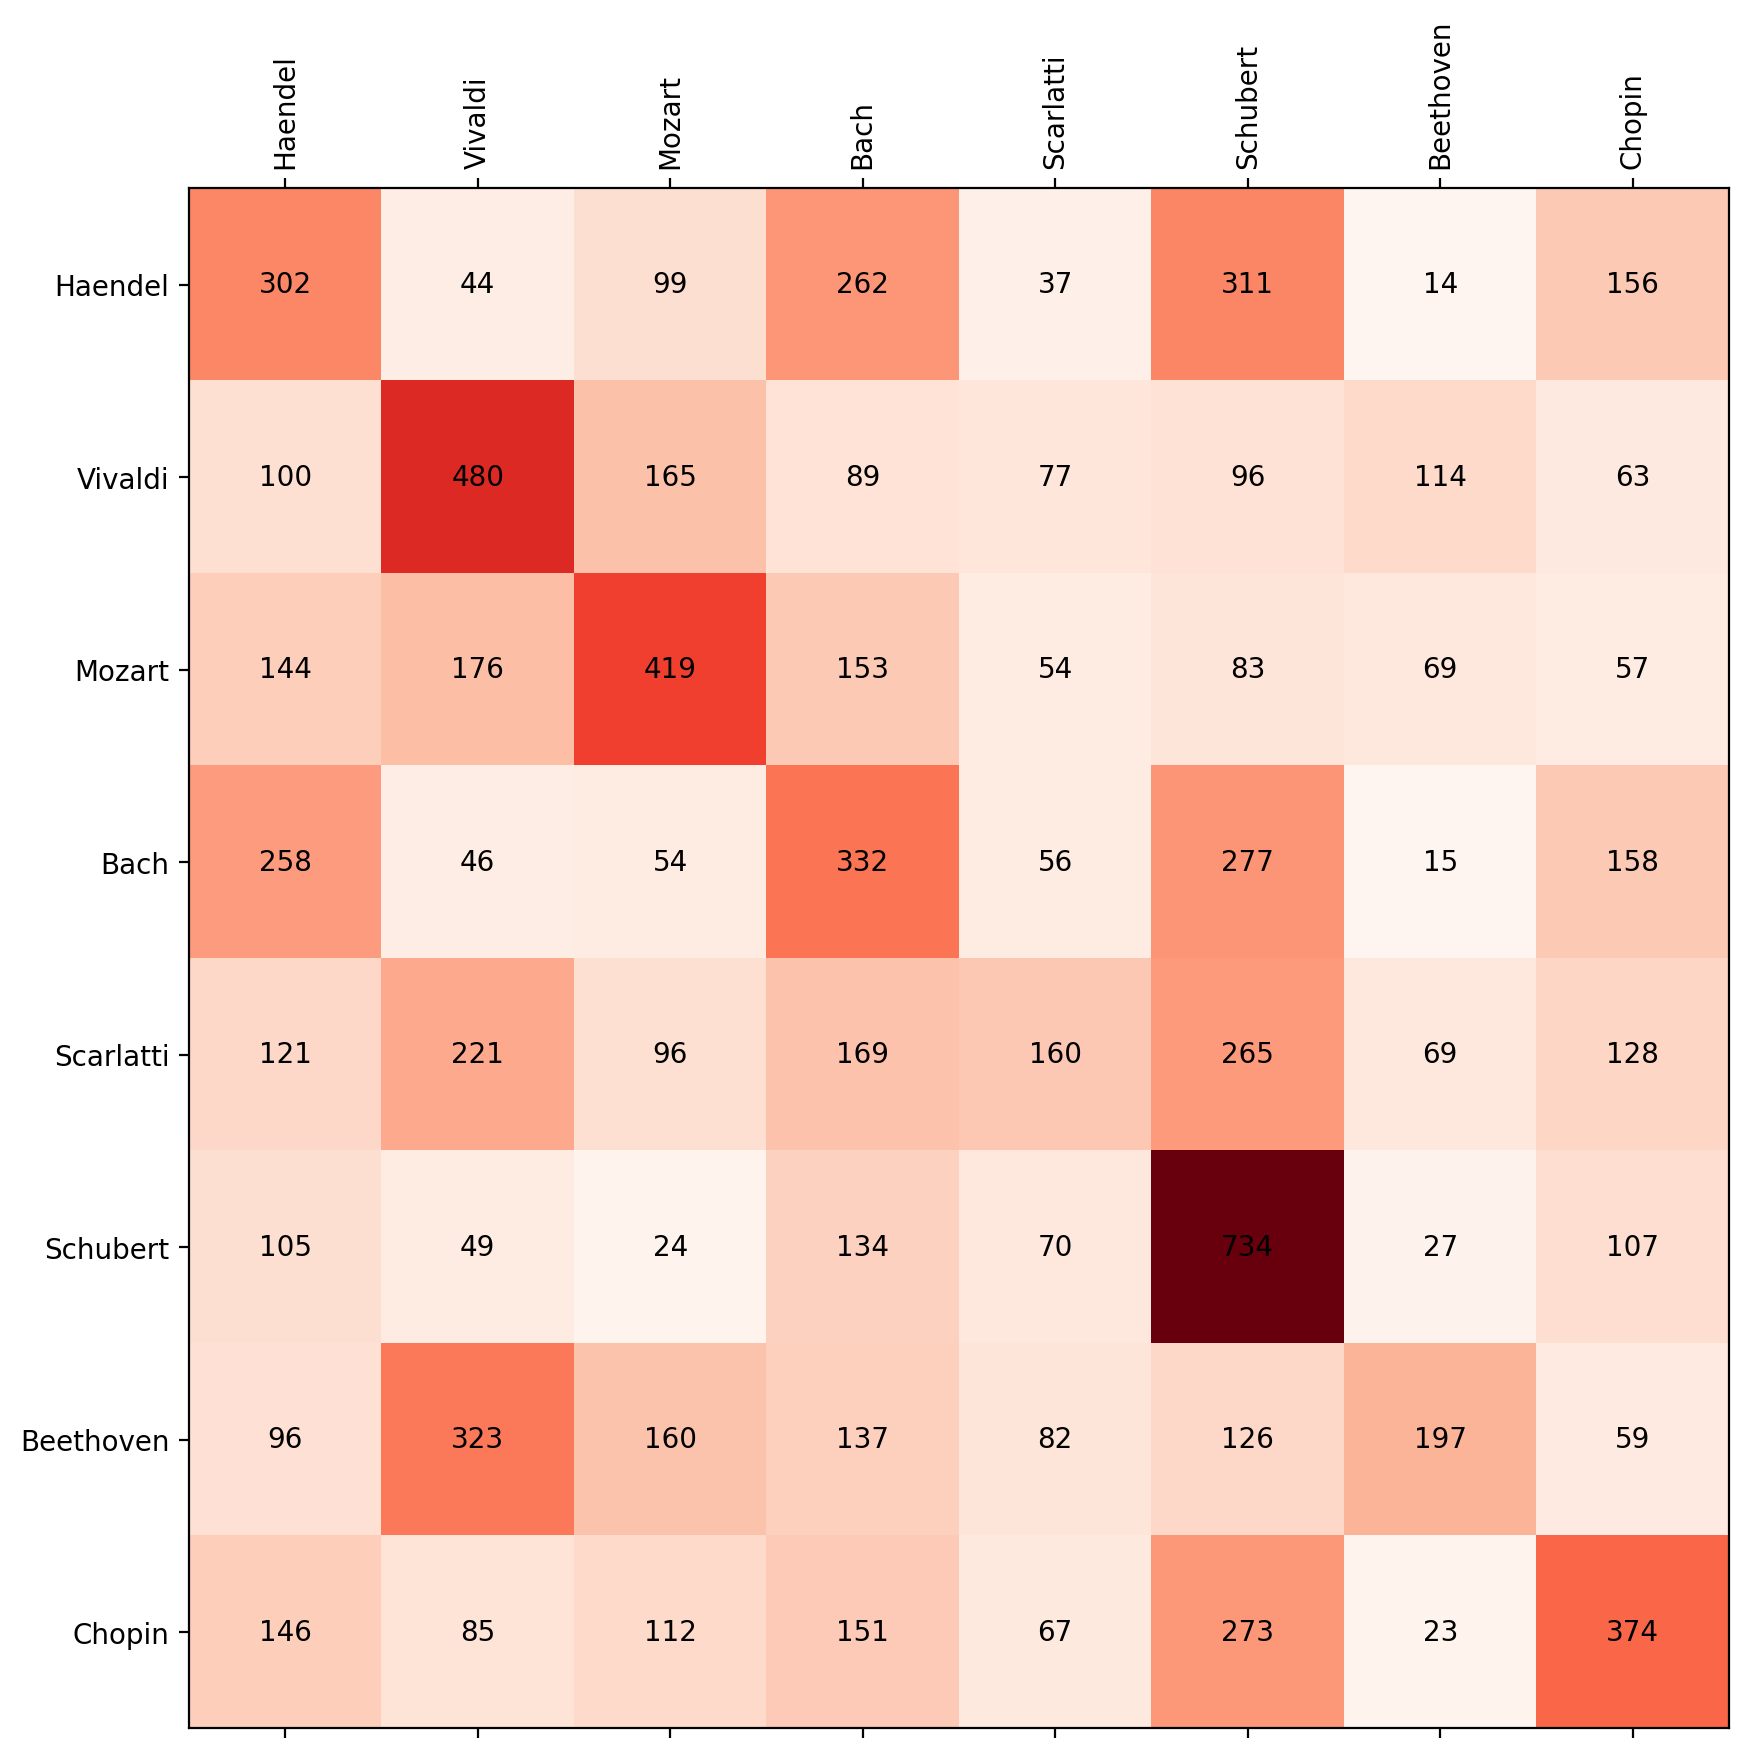
\includegraphics[width=1\textwidth]{Klassifikation_ohne_Epochen.png}
  \caption{Klassifikation mit 1.000 Bäumen im Forest}
  \label{fig:Klassifikation_ohne_Epochen}
\end{figure}

Das Problem, wenn man \emph{n\_estimators} höher setzt, ist, dass es länger braucht zum Laden. Durch die Beobachtung, dass Werke, die der gleichen Epoche angehören öfter verwechselt werdenn, sind wir
auf die Idee gekommen im zweiten Versuch über zwei (bzw. dann fünf) Modelle zu klassifizieren. Hier haben wir zuerst das Lied seiner Epoche und dann innerhalb dieser dem Komponisten zugeordnet.


\subsection{Zweiter Versuch: Mit Einbezug der zeitlichen Epochen}
\subsubsection{Modell zur Klasssifizierung in die Epochen}
Wir trainieren zuerst nach den verschiedenen Epochen, in welchen die Künstler gelebt haben. Diese sind:
\begin{itemize}
    \item[Barock]: Scarlatti, Vivaldi, Bach, Haendel
    \item[Klassik]: Mozart, Beethofen
    \item[Romantik]: Schubert, Chopin
\end{itemize}

Die Accuracy beim Einordnen der Stücke in ihre jeweiligen Epochen beträgt 55\%. Auch hier verlieren wir wieder viele Daten, da bei der Zuordnung zu den verschiedenen Zeitabschnitten grosse Unterschiede
auftreten. So hat die Epoche Barock 61.051 Stücke, während es in der Romantik nur noch 23.013 gibt. Also verlieren wir beim Balancieren der Datensets 1/3 der Daten. Was zwar nicht so schlimm, wie beim 
ersten Versuch (bei welchem wir fast 80\% verloren haben), aber trotzdem nicht gut ist. Auch das können wir später wieder erkennen.

\subsubsection{Modelle zum Klassifizieren innerhalb der einzelnen Epochen}
Innerhalb der verschiedenen Epochen (Barock, Klassik und Romantik) werden die Werke ihren Komponisten zugeordnet. Das hat, wie man in der Grafik \ref{fig:Innerhalb_der_Epochen} erkennen kann vorallem in der Klassik sowie Romantik
sehr gut funktiniert. Dort erreichen wir eine Accuracy von 67\% bzw. 66\% erreicht. Nur im Barock funktioniert es etwas schlechter mit einer Genauikgeit von 43\%, wobei vorallem Scarlatti und Vivaldi das
Problem ausmachen.

\begin{figure}[h]
  \centering
  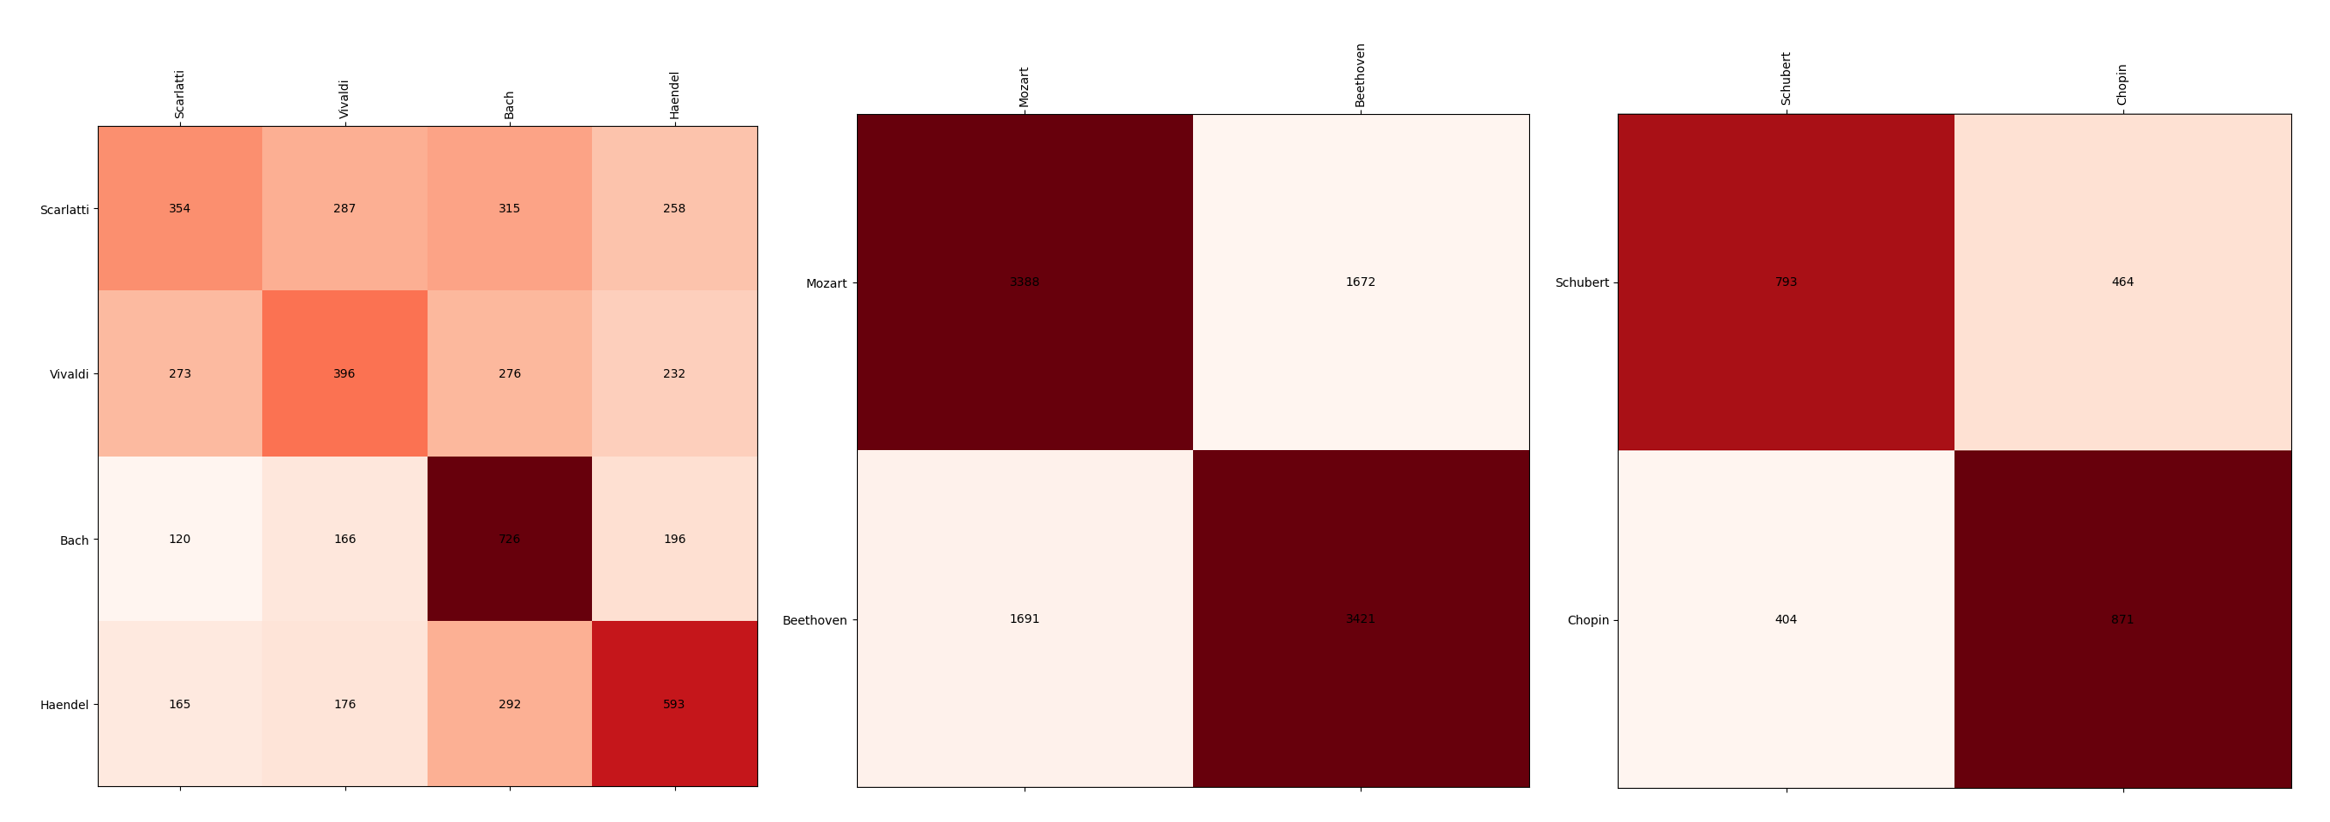
\includegraphics[width=1\textwidth]{Innerhalb_der_Epochen.png}
  \caption{Links: Barock, Mitte: Klassik, Recht: Romantik}
  \label{fig:Innerhalb_der_Epochen}
\end{figure}

\subsubsection{Verbinden der Modelle}
Schlussendlich haben wir diese vier Modelle in folgendem Sinne verbunden:

\begin{figure}[h]
  \centering
  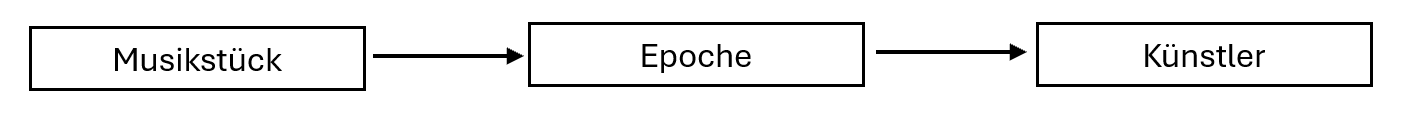
\includegraphics[width=1\textwidth]{Verbinden_der_Modelle.png}
  \caption{Verbinden der Modelle}
  \label{fig:Verbinden_der_Modelle}
\end{figure}

Wie man im Flowchart \ref{fig:Verbinden_der_Modelle} entnehmen kann, wird ein Musikstück genommen und seiner Epoche zugeordnet. Innerhalb dieser Epoche wird es dann wieder seinem Künstler zugeteilt.
Mit diesen fünf Modellen haben wir eine Accuracy von knapp 40\% erreicht, was auch nicht gut ist.
Dies liegt wahrscheinlich daran, dass schon beim Einteilen in die verschiedenen Epochen nur eine Genauigkeit von 55\% erreicht werden kann. Somit wäre das dann auch die maximal mögliche Genauigkeit.
Man könnte diese durch Datenaugumentation erhöhen, indem man nicht die Stücke aus der Barockepoche wegschneidet, sodass man gleichviele hat, wie in der Romantik. Sondern so viele in der Romantik hinzugibt, bis die Anzahl ähnlich ist.
Das haben wir in Versuch 3 umgesetzt:

\subsection{Versuch 3: Balancieren mittels Datenaugumentation}


\end{document}